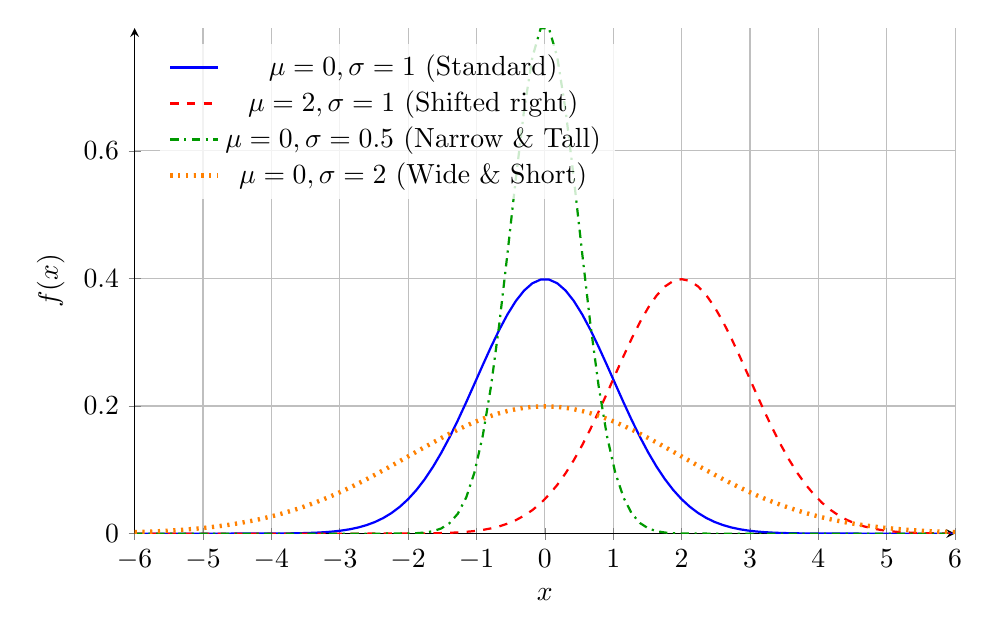
\begin{tikzpicture}
\begin{axis}[
    width=12cm,
    height=8cm,
    domain=-6:6,
    samples=100,
    axis lines=left,
    xlabel={$x$},
    ylabel={$f(x)$},
    grid=major,
    legend pos=north west,
    legend style={draw=none, fill=white, fill opacity=0.8, text opacity=1},
    every axis plot/.append style={thick}
]

% 1. Standard Normal: mu=0, sigma=1
\addplot [blue] 
    {exp(-x^2/2) / sqrt(2*pi)};
\addlegendentry{$\mu=0, \sigma=1$ (Standard)}

% 2. Shifted mean: mu=2, sigma=1
\addplot [red, dashed] 
    {exp(-(x-2)^2/2) / sqrt(2*pi)};
\addlegendentry{$\mu=2, \sigma=1$ (Shifted right)}

% 3. Smaller standard deviation (narrow/tall): mu=0, sigma=0.5
\addplot [green!60!black, dashdotted] 
    {exp(-x^2/(2*0.5^2)) / (0.5*sqrt(2*pi))};
\addlegendentry{$\mu=0, \sigma=0.5$ (Narrow \& Tall)}

% 4. Larger standard deviation (wide/short): mu=0, sigma=2
\addplot [orange, dotted, ultra thick] 
    {exp(-x^2/(2*2^2)) / (2*sqrt(2*pi))};
\addlegendentry{$\mu=0, \sigma=2$ (Wide \& Short)}

\end{axis}
\end{tikzpicture}